\section{Theory}

\subsection{Electroencephalography (EEG)}

    Electroencephalography is a method used to measure the activity of neurons in the brain by recording the electrical activity on the scalp.

    As a non-invasive method it is widely used in medicine to diagnose and study a wide range of conditions, from epilepsy to sleep disorders.

    In research it has also found use in studying ``Event Related Potentials'', or ERPs, which are stereotypes responses to a stimulus. Common ERPs can be seen in Table~\ref{table:erps}.

    \begin{table}
        \begin{tabular}{ll}
            \toprule
            ERP & Description
            \\
            \midrule
            N170 & Elicited by processing of faces, familiar objects or words.
            \\
            N400 & Elicited by words and other stimuli.
            \\
            P600 & Elicited by hearing or reading grammatical errors and other syntactic anomalies.
            \\
            \bottomrule
        \end{tabular}
        \caption{Common ERPs}\label{table:erps}
    \end{table}

    Electrodes can be placed at different locations on the scalp, targeting different regions of the brain. The system used to position the electrodes is called the 10–20 system, and is the standard way to label electrode placements.

    \begin{figure}
        \begin{center}
            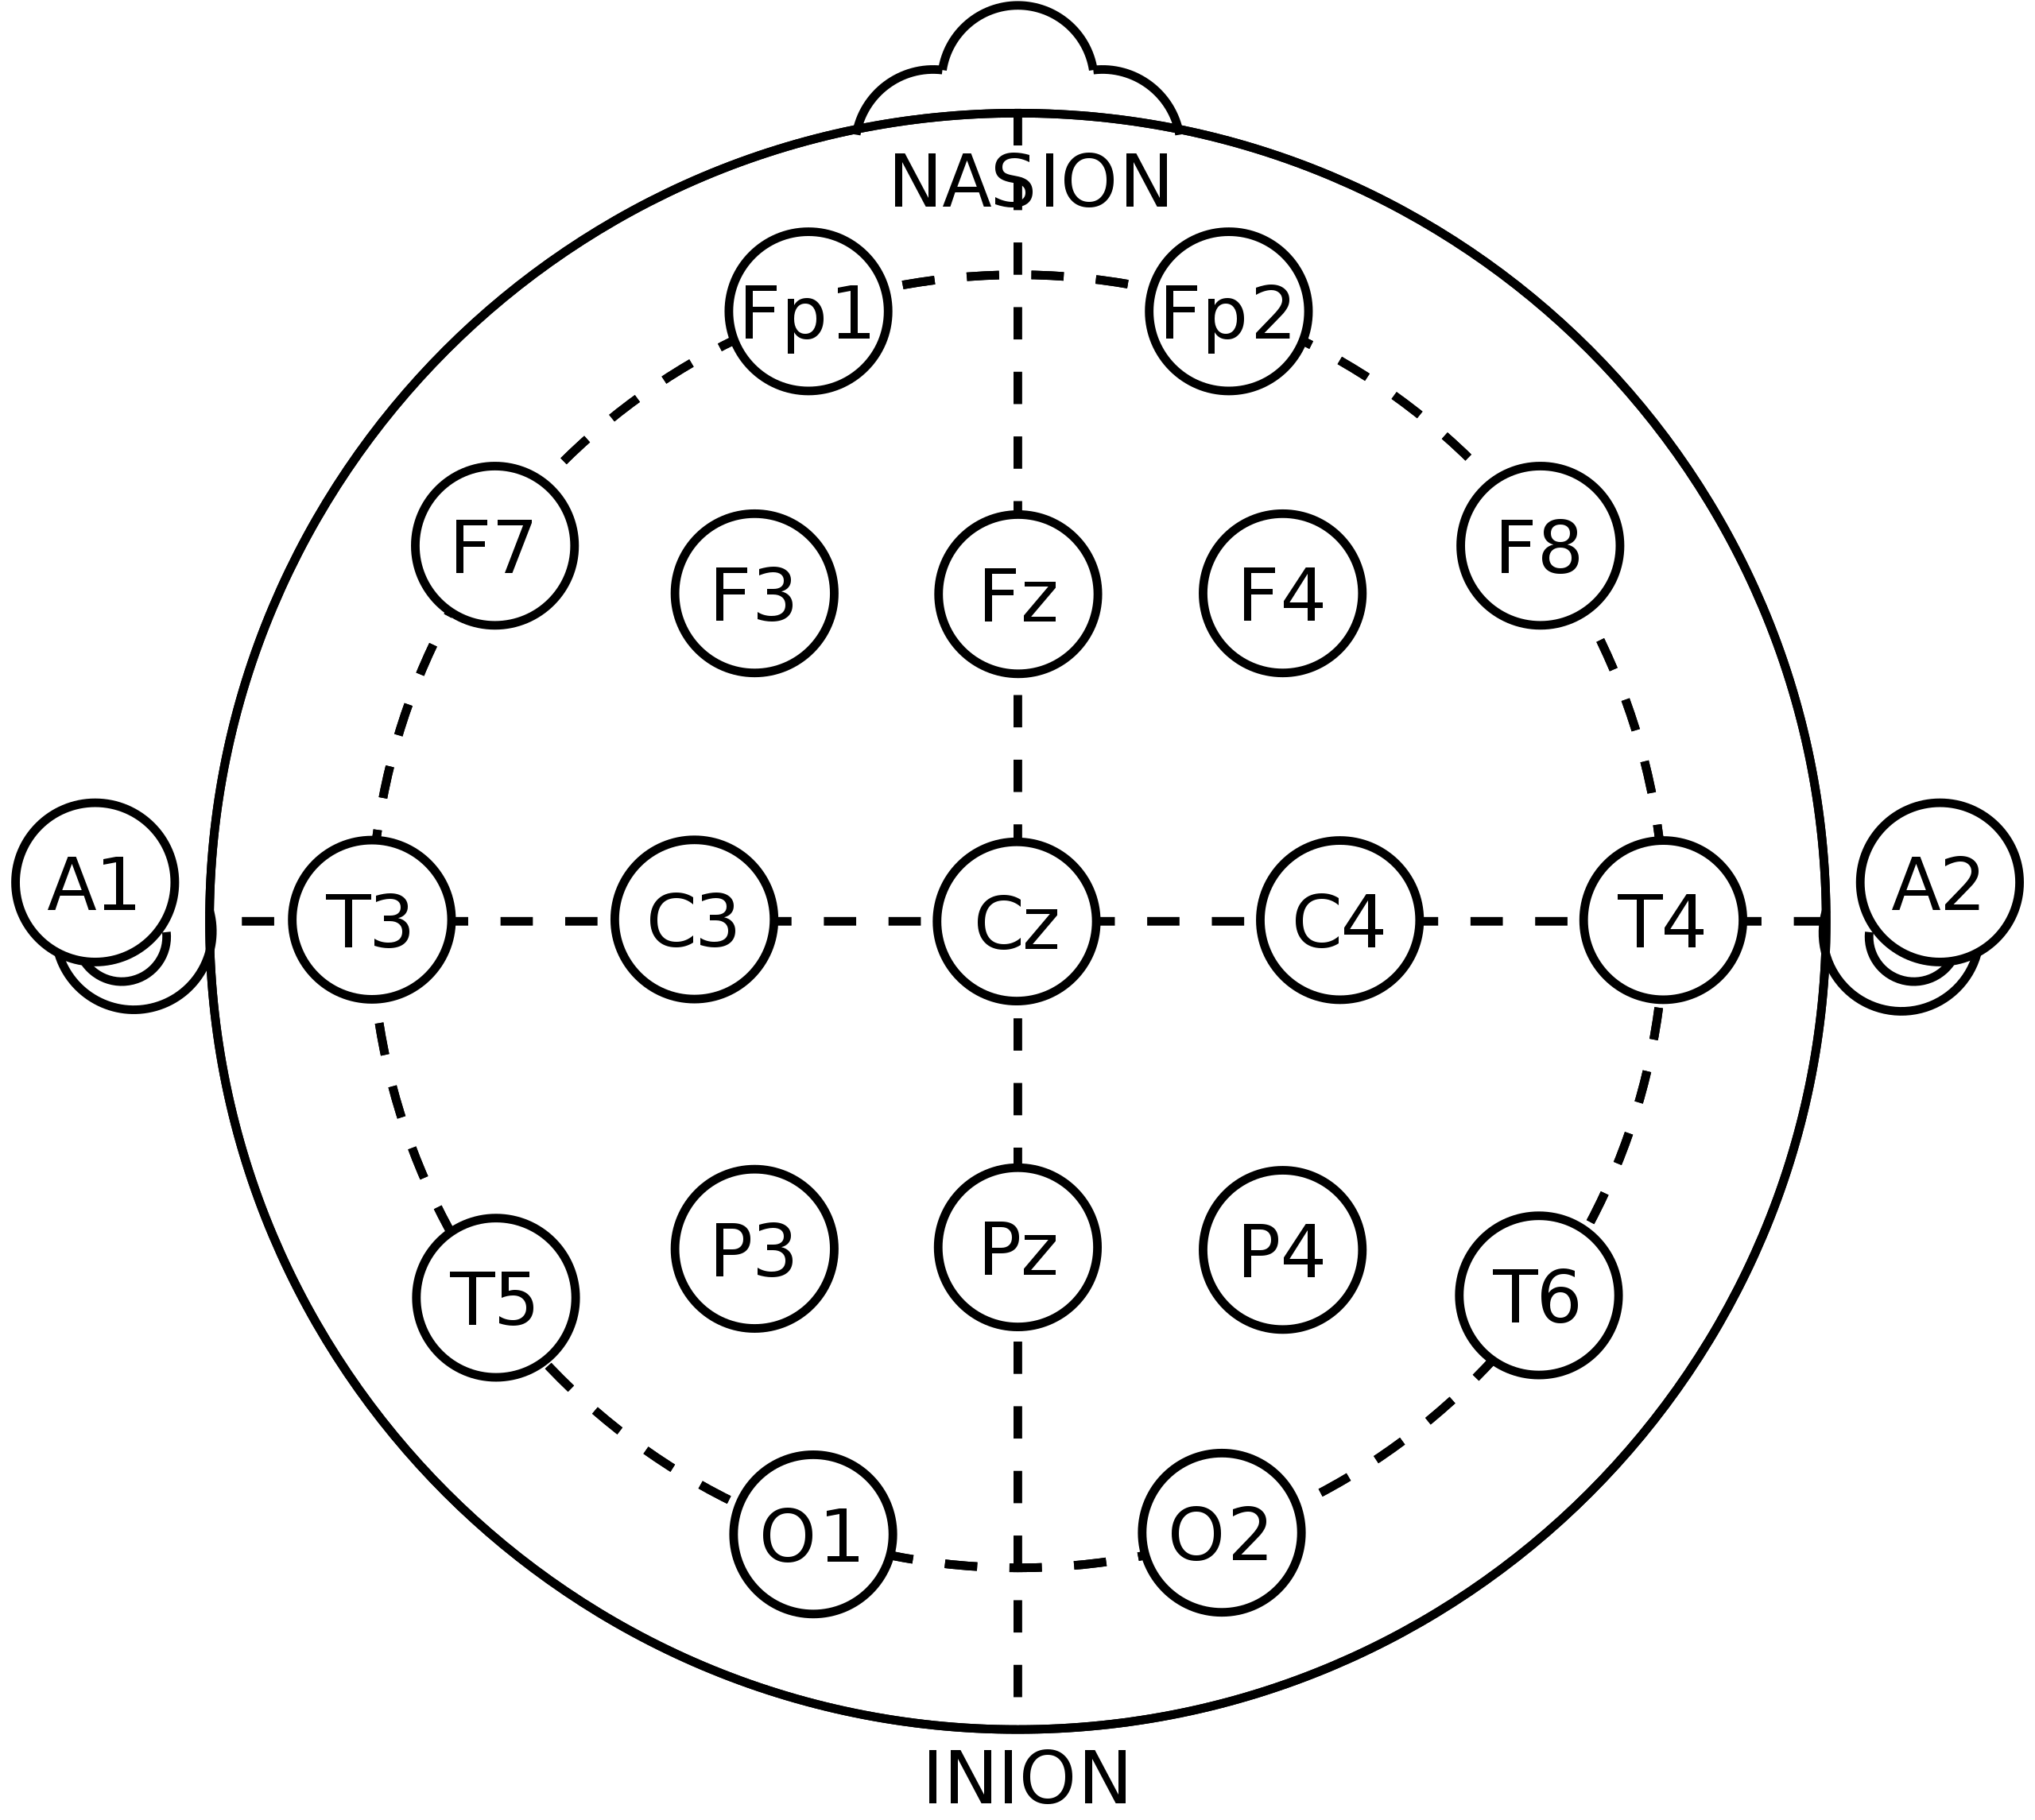
\includegraphics[width=10cm]{img/1020 system.png}
        \end{center}
        \caption{The 10–20 system}\label{fig:1020}
    \end{figure}

    \add[inline]{Explain theory used, like theory of EEG, Riemannian geometry, etc}
    \add[inline]{Plots of raw EEG signal, PSD, PCA, etc}

    As measurements are taken on the scalp, neural activity of surface-level neurons can be expected to dominate the signal, which makes it difficult to use when studying systems deeper in the brain, such as the hippocampus. As an example of this, eye blinks are easily identifieable in the signal when electrodes are placed on the frontal cortex.

    \add[inline]{Mention need for bandpass filtering to get rid of powerline noise}

    \add[inline]{Plot of signal during eye blink}
    \add[inline]{Discuss some of the review articles on EEG/BCI/ML}

\subsection{Machine Learning}

    Machine learning on EEG data utilizes several domain-specific methods (which?) often similar to other methods seen applied to general time-series data.

    Among these we find methods like bandpass filtering, windowing, spectral density estimation, and the computation of covariance matrices to find interdependencies between channels.

    Common methods used in analysis and classification of EEG data include Linear Discriminant Analysis (LDA), Common Spatial Pattern (CSP) filters.

    With the use of these methods, we can compute features to use when training our classifiers.

    The underlying ML algorithms themselves are often off-the-shelf logistic regression, with some domain adaptations found in more complex models like neural networks.

    \add[inline]{Formulas}

    \subsubsection{Riemannian geometry}

        \add[inline]{Explanation of Riemannian geometry, from \href{https://colab.research.google.com/drive/1y9tq7-lJwusxtVgpB38y-p1pYw7hg0iu}{this tutorial we're working on}, perhaps it should go in the Background/Theory section though?}

